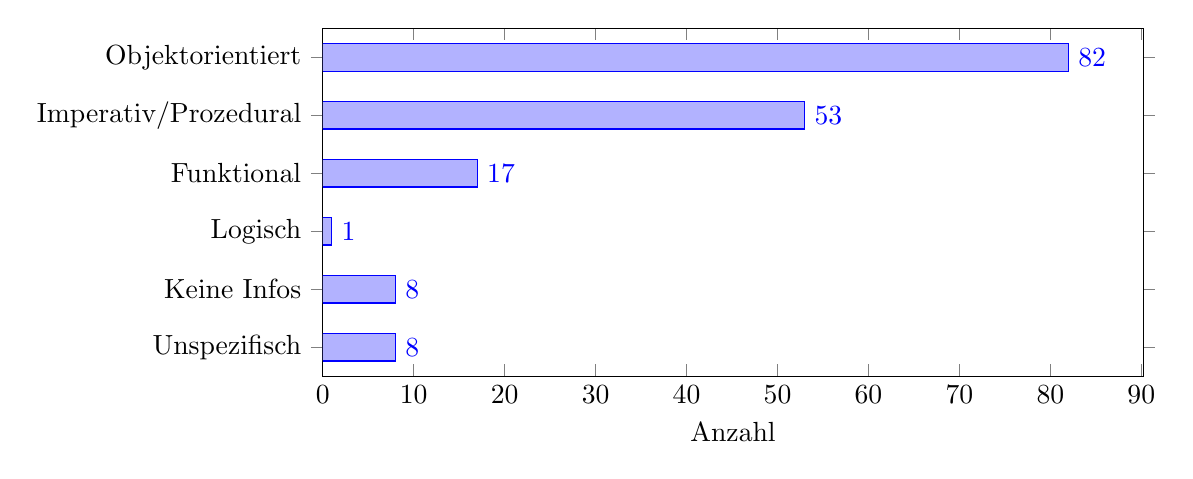
\begin{tikzpicture}
    \begin{axis}[
        xbar,
        width=12cm,
        height=6cm,
        symbolic y coords={{Unspezifisch}, {Keine Infos}, {Logisch}, {Funktional}, {Imperativ/Prozedural}, {Objektorientiert}},
        ytick=data,
        nodes near coords,
        xmin=0,
        xlabel={Anzahl}
    ]
        \addplot coordinates {
            (8,{Unspezifisch}) (8,{Keine Infos}) (1,{Logisch}) (17,{Funktional}) (53,{Imperativ/Prozedural}) (82,{Objektorientiert})
        };
    \end{axis}
\end{tikzpicture}